\documentclass[solution, letterpaper]{cs124}
\usepackage{dsfont}

%% Please fill in your name and collaboration statement here.
\newcommand{\studentName}{**NICK STANFORD**}
\newcommand{\collaborationStatement}{**I collaborated with Julia Winn, Billy Cember, and Lexi Ross**}

\begin{document}

\header{1}{Tuesday, February 7, 2012}


\setcounter{Part}{1}
 \begin{center}
Nick Stanford Jackie Quinn
 \end{center}

\problem{} 
Give a dynamic programming solution to the Number Partition problem.

\subsolution


We will be dealing with a $n$ by $b$ matrix. As stated in the problem, $n$ is the number of elements in the set and $b$ is the sum of all of the elements in the set. Conceptually we want the ith jth entry $P(i,j)$ to equal one if it is possible to sum to j using only $s_1 ... s_i$ and zero otherwise. The following recurrence captures this:

$$P(i,j) = \max{\{P(i-1,j), P(i-1,j-s_i)\}} $$

When the matrix is totally filled in, we look at the bottom row. This represents all of the possible sums that can be reached using a subset of the elements in S. We scan this line, looking for the element closest in value to $\frac{b}{2}$. Call it $A$. The residue is then $2A-b$.

Running time: we fill in $nb$ squares, each of which is constant time. $O(nb)$. 

\problem{} 
Explain briefly how the Karmarkar-Karp algorithm can be implemented in O(nlogn) steps, assuming the values in A are small enough that arithmetic operations take one step.

\subsolution Take your set of values and sort it in $O(n \log{n})$ time. Then pull off the top two elements. Do the differencing, discard the zero, and insert the difference back into the sorted list. This takes $O(\log{n})$ time. Each time we take a difference, we discard an element. Therefore, we repeat this $n$ times. This gives a running time of

$$ n \log{n} + n \log{n} = O(n\log{n}) $$

\problem{}
Discuss your results:

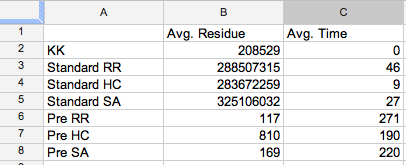
\includegraphics[scale=0.50]{PA3results} \\

\subsolution Across the board, the solutions which used the prepartition representation performed much better than those which used the standard representation. This is to be expected. Firstly, the random algorithms using prepartitioning incorporate KK when calculating their residues. We know that KK is an effective characteristic, so its inclusion in all of the prepartioning algorithms gives it an advantage over standard representation. The implication is that the prepartition solutions aren't random in the same way that the standard representation are. It is possible to get a random standard solution with a pretty bad residue. It is a lot harder to get a really high residue with the standard appraoch because the KK heuristic is still applied and figures out a good way to split the sets. 

I would expect the KK algorithm to work better on sets whose elements were smaller relative to the number of elements in the set. The differencing operation effectively decides to put two elements in different sets without signifying which set specifically. You can imagine that the strategy of putting the two largest elements available into seperate sets would break down as the potential size difference between them gets huge. In our experiments, the ratio of the elements is $10^10$. The increased performance of the random prepartition algorithms over regular KK can be attributed to the 25,000 repetitions they go through. Smaller answers will eventually emerge. 

One surprise was the relatively lack of difference between the random, hill-climbing and simulated annealing solutions. The best solution that hill climbing can find is the local minima of the solution space that the first random solution happened to fall into. Random and simulated annealing don't have this problem, as they can jump out of minima wells and find other minima. Also, as the number of reptitions goes to infinity random guessing should converge on the ideal solution (because in infinite trials it samples all of the solution space). This is also true to a lesser extent for simulated annealing (as the trial number increases, it becomes harder, but not impossible, to escape the minima you are currently in). Therefore, given a sufficiently large number of trials, we would expect pure random to do the best, followed by siulated annealing, followed by hill-climbing. 

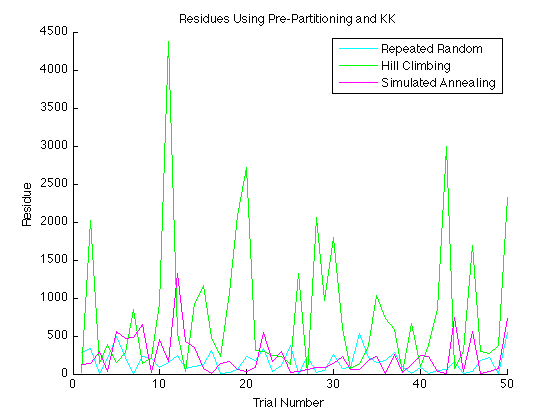
\includegraphics[scale=0.50]{fig-res-pre.png}
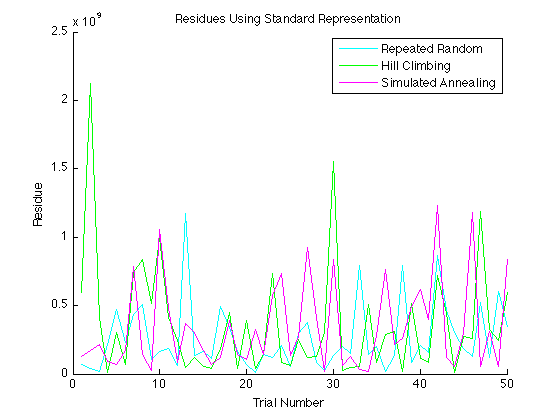
\includegraphics[scale=0.50]{fig-res-stand.png}\\
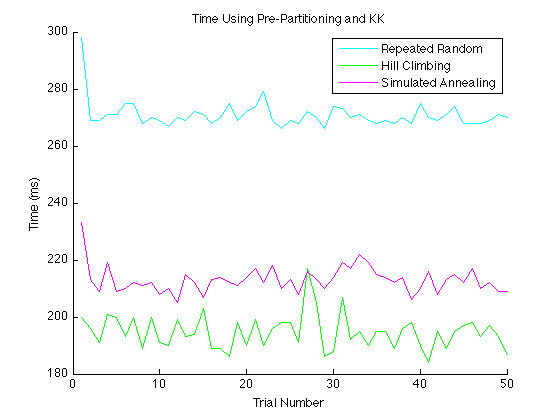
\includegraphics[scale=0.50]{fig-time-pre.png}
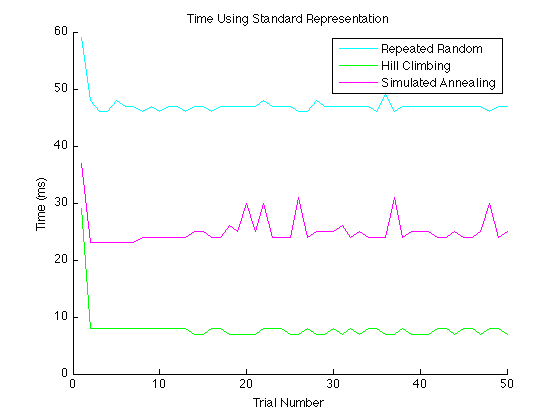
\includegraphics[scale=0.50]{fig-time-stand.png}


\problem{}
We know that the solution to the Karmarcher-Karp algorithm isn't perfect. If we start from a solution from KK, we can use simulated annealing to move around the solution state and possibly find a more ideal solution. The problem with simulated annealing is getting close to this solution in the first place. There will be less "bad" solution space to have to dig through. 



%%%%%%%%%%%%%%%%%%%%%%%%%%%%%%%%%%%%%%%%%%%%%%%%%%%%%%%%%%%%%%%%%%%%%%%%%%%%%%

\end{document}